% Source of docs/methodology.pdf.
% Figures: python docs/methodology_src/make_figures.py   (writes figs/; needs the stitched E2a hindcast)
% Build:   tectonic -X compile docs/methodology_src/methodology.tex --outdir <tmp> && cp <tmp>/methodology.pdf docs/
%          (tectonic is in the conda env `docs-build`; no system LaTeX is installed on this machine)
\documentclass[11pt,a4paper]{article}
\usepackage[margin=2.3cm]{geometry}
\usepackage[T1]{fontenc}
\usepackage{lmodern}
\usepackage{microtype}
\usepackage{amsmath,amssymb}
\usepackage{booktabs}
\usepackage{graphicx}
\usepackage{xcolor}
\usepackage{tikz}
\usetikzlibrary{positioning,arrows.meta,fit,calc}
\usepackage{caption}
\usepackage{enumitem}
\usepackage[round]{natbib}
\usepackage[hidelinks]{hyperref}
\usepackage{array}

\definecolor{ink}{HTML}{1B1B1B}
\definecolor{ink2}{HTML}{52514E}
\definecolor{accent}{HTML}{2A78D6}
\definecolor{accent2}{HTML}{EB6834}
\definecolor{wash}{HTML}{EEF3FA}
\hypersetup{colorlinks=true,linkcolor=accent,urlcolor=accent,citecolor=accent}
\captionsetup{font=small,labelfont=bf}
\setlist{itemsep=2pt,topsep=4pt}
\graphicspath{{figs/}}

\newcommand{\HM}{\mathrm{HM}}
\newcommand{\code}[1]{\texttt{\small #1}}
\newcommand{\E}{\mathbb{E}}

\title{\textbf{Probabilistic projections of human modification of the\\ terrestrial biosphere from 2020 to 2040}\\[6pt]
\large Technical methodology of the forecasting model (production model E2a)}
\author{}
\date{Technical companion to the manuscript of Moncrieff et al.\\[2pt]
\small Prepared 25 September 2026 from repository \code{spatio-temporal}, branch \code{main}}

\begin{document}
\maketitle
\thispagestyle{empty}

\begin{abstract}
\noindent
This document specifies, at implementation level, the model that produces the global Human
Modification (HM) forecast and hindcast products. A convolutional LSTM encodes a three-step
history of HM and its stressor, socio-economic, climatic and neighbourhood covariates on a
$\sim$1\,km global grid. For each of four horizons (+5, +10, +15 and +20 years) it emits a
monotone piecewise-linear quantile function per pixel. The whole predictive distribution is the
product; no ensemble, recalibration or post-hoc reshaping follows the network. Training
minimises the continuous ranked probability score (CRPS), evaluated in closed form. Skill is
measured out of sample with five-fold spatial-block cross-validation over all
184,573,321 scored land pixels. Every number, formula and setting below was taken from the code,
the checkpoints, or the logs of the production run; where the implementation departs from what
one might assume, the document says so. It is the technical companion to the manuscript, whose
Methods describe the approach without implementation detail; terminology follows the manuscript.
\end{abstract}

\setcounter{tocdepth}{1}
\tableofcontents
\newpage

%=====================================================================================
\section{Overview}
%=====================================================================================

\paragraph{Task.} Given HM at three past dates $(t-10,\,t-5,\,t)$ together with covariates,
predict the full distribution of HM at $t+5$, $t+10$, $t+15$ and $t+20$ at every land pixel of
a global grid. HM quantifies the cumulative impact of 16 anthropogenic threats, grouped into eight thematic
classes that map to the IUCN threat taxonomy, as a continuous index on $[0,1]$. It is available
every five years from 1990 to 2020 \citep{theobald}; its change over twenty years is small almost everywhere (the median 20-year
change is 0.0001) and heavily right-skewed where it happens.

\paragraph{Products.} Two products are built from one model configuration:
\begin{itemize}
\item a \textbf{hindcast}, base year 2000 (inputs 1990, 1995, 2000; targets 2005, 2010, 2015,
  2020). It is a mosaic of five cross-validation models in which every pixel is predicted by the
  model that never trained on it, so it is out of sample and is what the scores in
  Section~\ref{sec:eval} describe;
\item a \textbf{forecast}, base year 2020 (inputs 2010, 2015, 2020; targets 2025, 2030, 2035,
  2040), from a single model trained on all data.
\end{itemize}
Each is delivered as Cloud-Optimised GeoTIFFs (lower, mean, upper, $P(\HM>0.1)$,
$P(\HM>0.4)$ per year) and as an icechunk store holding all 64 quantile levels per pixel
(Section~\ref{sec:global}).

\paragraph{The production model, E2a.} The network (Figure~\ref{fig:arch}) has three parts.
\begin{enumerate}
\item A \emph{location encoder} maps longitude and latitude to 8 features
  (Section~\ref{sec:locenc}).
\item A four-layer \emph{ConvLSTM trunk} with 64 hidden channels reads a 38-channel input at
  each of three time steps (Section~\ref{sec:trunk}).
\item Per horizon, two small convolutional \emph{heads} emit 15 numbers per pixel: a location
  (the median) and 14 positive increments that define a piecewise-linear quantile function on a
  fixed grid of 15 quantile levels (Section~\ref{sec:heads}).
\end{enumerate}
The network has 1,355,588 trainable parameters on the production path. It is trained end to end
on the CRPS alone (Section~\ref{sec:loss}).

\paragraph{How E2a was chosen.} Twenty-three configurations of the distributional head were
screened on Africa (63.1\,Mpx, two folds, one seed each), varying the interpolating family, knot
grid, width parameterisation and tail treatment. The two finalists were run globally with the
full five-fold protocol:
\begin{itemize}
\item \textbf{E1v}, a 17-parameter head with two learned exponential tail rates;
\item \textbf{E2a}, the same head without them (15 parameters).
\end{itemize}
Centrally they are indistinguishable. Far from past change, E2a is sharper and its point forecast
beats persistence, while its intervals are too narrow there (Section~\ref{sec:ab}). E2a was chosen
as the production model on 25 September 2026.

\begin{figure}[t]
\centering
\resizebox{\linewidth}{!}{%
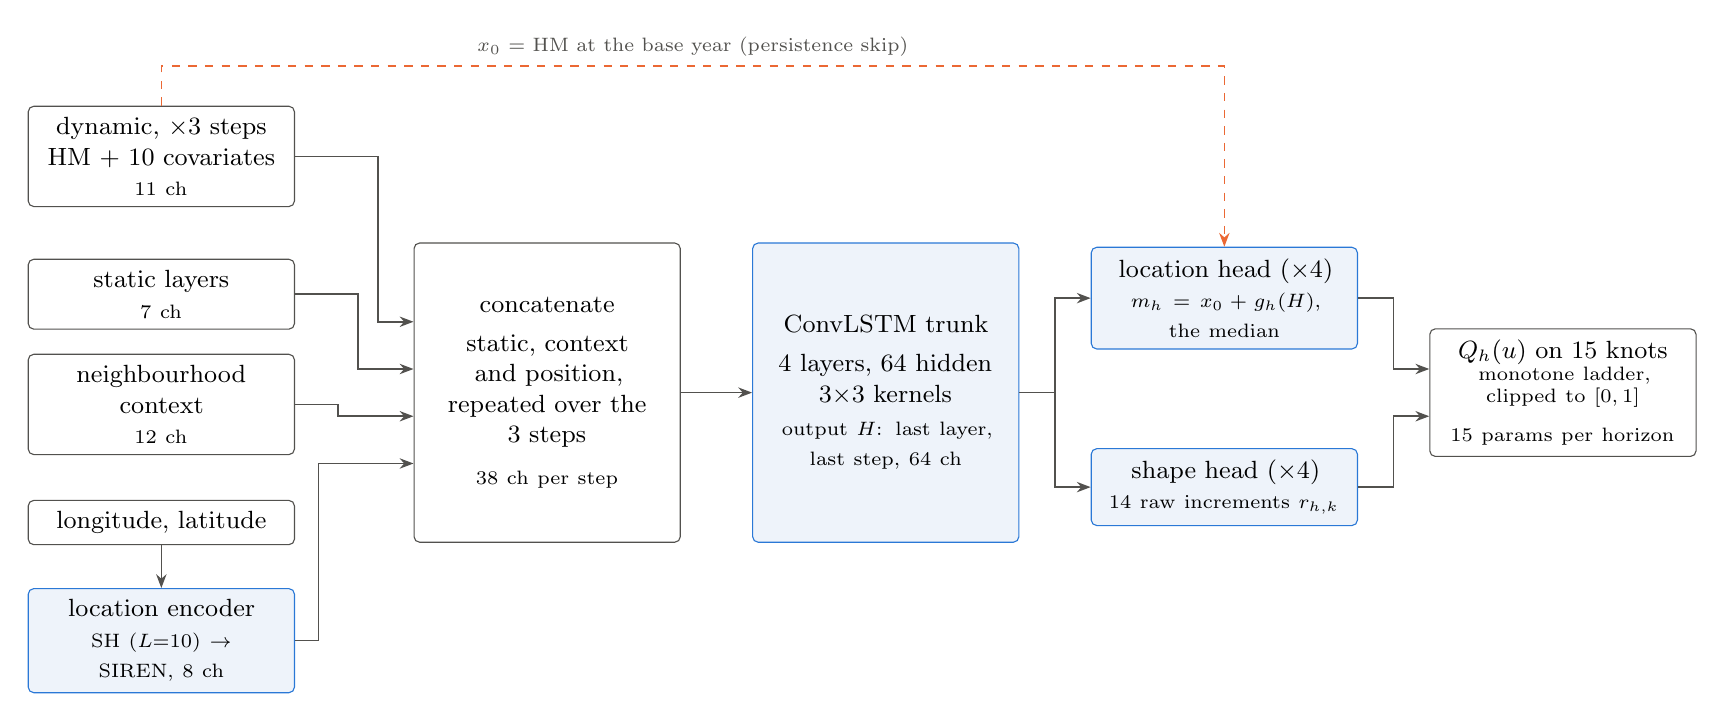
\begin{tikzpicture}[
  font=\small,
  box/.style={draw=ink2, rounded corners=2pt, align=center, inner sep=4pt, fill=white, text width=31mm},
  hl/.style={box, fill=wash, draw=accent},
  arr/.style={-{Stealth[length=5pt]}, draw=ink2, line width=0.6pt}]
% inputs, column 1
\node[box] (dyn) at (0, 3.7)  {dynamic, $\times$3 steps\\ HM + 10 covariates\\ \scriptsize 11 ch};
\node[box] (sta) at (0, 1.95) {static layers\\ \scriptsize 7 ch};
\node[box] (ctx) at (0, 0.55) {neighbourhood context\\ \scriptsize 12 ch};
\node[box] (ll)  at (0,-0.95) {longitude, latitude};
\node[hl]  (le)  at (0,-2.45) {location encoder\\ \scriptsize SH ($L{=}10$) $\to$ SIREN, 8 ch};
% concat and trunk
\node[box, minimum height=38mm] (cat) at (4.9, 0.7) {concatenate\\[3pt] static, context and position,\\ repeated over the\\ 3 steps\\[4pt] \scriptsize 38 ch per step};
\node[hl, minimum height=38mm] (trunk) at (9.2, 0.7) {ConvLSTM trunk\\[3pt] 4 layers, 64 hidden\\ $3{\times}3$ kernels\\[4pt] \scriptsize output $H$: last layer,\\ \scriptsize last step, 64 ch};
% heads and output
\node[hl] (loc) at (13.5, 1.9) {location head ($\times$4)\\ \scriptsize $m_h = x_0 + g_h(H)$, the median};
\node[hl] (shp) at (13.5,-0.5) {shape head ($\times$4)\\ \scriptsize 14 raw increments $r_{h,k}$};
\node[box] (q) at (17.8, 0.7) {$Q_h(u)$ on 15 knots\\ \scriptsize monotone ladder,\\ \scriptsize clipped to $[0,1]$\\[3pt] \scriptsize 15 params per horizon};
% arrows: each input gets its own lane into the concatenation
\draw[arr] (dyn.east) -- ++(1.05,0) |- ([yshift=9mm]cat.west);
\draw[arr] (sta.east) -- ++(0.80,0) |- ([yshift=3mm]cat.west);
\draw[arr] (ctx.east) -- ++(0.55,0) |- ([yshift=-3mm]cat.west);
\draw[arr] (le.east)  -- ++(0.30,0) |- ([yshift=-9mm]cat.west);
\draw[arr] (ll) -- (le);
\draw[arr] (cat) -- (trunk);
\draw[arr] (trunk.east) -- ++(0.45,0) |- (loc.west);
\draw[arr] (trunk.east) -- ++(0.45,0) |- (shp.west);
\draw[arr] (loc.east) -- ++(0.45,0) |- ([yshift=3mm]q.west);
\draw[arr] (shp.east) -- ++(0.45,0) |- ([yshift=-3mm]q.west);
\draw[arr, dashed, draw=accent2] (dyn.north) -- ++(0,0.5) -| node[pos=0.25, above, font=\scriptsize, text=ink2]
  {$x_0$ = HM at the base year (persistence skip)} (loc.north);
\end{tikzpicture}}
\caption{The E2a network. Channel counts are per time step. The dashed path adds the base-year
HM to the location head's output, so the untrained model forecasts persistence. Per horizon the
output is 1 location + 14 increments = 15 parameters per pixel.}
\label{fig:arch}
\end{figure}

\paragraph{Notation.} $x_0$ is HM at the base year $t$; $y_h$ is observed HM at $t+h$;
$Q_h(u)$ is the predicted quantile function at horizon $h\in\{5,10,15,20\}$ years and
$F_h = Q_h^{-1}$ its CDF; $u\in[0,1]$ is a quantile level; $\mu_{\HM}$ and $\sigma_{\HM}$ are the
HM normalisation constants (Section~\ref{sec:transform}). The model works internally in
normalised units $z = (\HM-\mu_{\HM})/\sigma_{\HM}$, and everything reported is back-transformed
to HM.

%=====================================================================================
\section{Input data}
\label{sec:data}
%=====================================================================================

\paragraph{Grid.} All rasters share one grid: EPSG:4326, $40000\times17111$ pixels at
$0.009^\circ$ ($\approx$1\,km at the equator), spanning $180^\circ$W--$180^\circ$E and
$83.997^\circ$N--$70.002^\circ$S. Of its 684.4\,M pixels, 184.6\,M are land with valid HM.
Nothing is resampled or reprojected at any stage.

\paragraph{Variables.} Table~\ref{tab:inputs} lists every input.
\begin{itemize}
\item \emph{Response.} Cumulative HM (\code{AA}) from \citet{theobald}, produced at 300\,m and
  average-resampled to the 1\,km grid.
\item \emph{HM component threats}, supplied individually as dynamic covariates: agriculture
  (\code{AG}), built environments (\code{BU}), extraction (\code{EX}), biological resource use
  (\code{FR}), human accessibility (\code{HI}), natural systems modification (\code{NS}),
  pollution (\code{PO}) and transportation (\code{TI}).
\item \emph{Socio-economic}, also dynamic: gridded population \citep{zhuang} and GDP
  \citep{murakami}, both aligned to the five-year HM years before they reach this repository.
\item \emph{Static}: elevation from EarthEnv, derived from GMTED2010 \citep{amatulli}; mean annual
  temperature (\code{tas}), minimum temperature of the coldest month (\code{tasmin}) and mean
  annual precipitation (\code{pr}) from CHELSA \citep{karger}; the Development Suitability Index
  (\code{dpi\_dsi}) \citep{oakleaf2024}; and two binary protected-area masks from the WDPA
  \citep{wdpa}, strictly protected (IUCN Ia, Ib, II; \code{iucn\_strict}) and all other
  categories (\code{iucn\_nostrict}), applied unchanged to every year.
\end{itemize}

\begin{table}[h]
\centering\small
\setlength{\tabcolsep}{4pt}\begin{tabular}{@{}llp{4.6cm}p{5.6cm}@{}}
\toprule
Group & Channels & Files & Content \\
\midrule
Target / dynamic & 1 & \code{HM\_\{year\}\_AA\_1000.tiff} & overall HM, $[0,1]$; also the first dynamic channel \\
Dynamic & 8 & \code{HM\_\{year\}\_\{v\}\_1000.tiff} & the eight HM component threats \code{AG, BU, EX, FR, HI, NS, PO, TI} \\
Dynamic & 2 & \code{HM\_\{year\}\_gdp/population} & gridded GDP \citep{murakami} and population \citep{zhuang} \\
Static & 7 & \code{hm\_static\_\{v\}\_1000.tiff} & elevation, three CHELSA climatologies, DSI, two WDPA protection masks \\
Context & 12 & \code{change\_context\_w\{t\}}, \code{hm\_context\_w\{t\}} & neighbourhood of past change and of current HM (Table~\ref{tab:context}) \\
Position & 8 & (computed) & location-encoder features from longitude and latitude \\
\bottomrule
\end{tabular}
\caption{Inputs. Dynamic channels are read at each of the three input dates; the others are read
once per sample and repeated across the three steps. Every time step therefore carries
$11+7+12+8=38$ channels.}
\label{tab:inputs}
\end{table}

\paragraph{Temporal windows.} A sample uses input dates $(t-10,t-5,t)$ and targets
$t+5,\dots,t+20$. HM exists only for 1990--2020, so the base year $t$ can be 2000, 2005, 2010 or
2015 during training, and horizons beyond 2020 are missing for the later bases:
\begin{center}\small
\begin{tabular}{@{}cccc@{}}
\toprule
base $t$ & inputs & observed targets & usable horizons \\
\midrule
2000 & 1990, 1995, 2000 & 2005, 2010, 2015, 2020 & 5, 10, 15, 20 \\
2005 & 1995, 2000, 2005 & 2010, 2015, 2020 & 5, 10, 15 \\
2010 & 2000, 2005, 2010 & 2015, 2020 & 5, 10 \\
2015 & 2005, 2010, 2015 & 2020 & 5 \\
\bottomrule
\end{tabular}
\end{center}
Missing targets are filled with NaN and masked out of the loss. The hindcast is predicted from
base 2000 and the forecast from base 2020.

%=====================================================================================
\section{Input data transformations}
\label{sec:transform}
%=====================================================================================

\paragraph{Missing values.} The HM rasters declare nodata as the \emph{finite} value
$3.4\times10^{38}$. Every reader uses a masked read, so the sentinel becomes NaN before any
arithmetic; an \code{isfinite} test on the raw values would instead count the ocean as fully
modified land. After that:
\begin{itemize}
\item the ten dynamic covariates have NaN set to 0 before normalisation, read as ``no pressure'';
\item static \code{ele}, \code{dpi\_dsi}, \code{iucn\_nostrict} and \code{iucn\_strict} have NaN
  set to 0 before normalisation; the climate layers keep their NaNs.
\end{itemize}

\paragraph{Normalisation.} Every channel except the context is standardised,
$\tilde v = (v-\mu_v)/\sigma_v$, with per-variable statistics:
\begin{itemize}
\item HM (input and target) uses one pooled mean and standard deviation over all seven years;
\item each covariate and static layer has its own mean and standard deviation.
\end{itemize}
The statistics are sample moments, ignoring NaN, of random $128\times128$ windows drawn with
seed 42: 37 windows per year for HM and for each dynamic covariate (259 each), and 37 per static
layer. $10^{-8}$ is added to each standard deviation. They are written once to
\code{data/conv\_spline/norm\_stats.json} and reused by every later run. They are \emph{not}
stored in the checkpoint, so prediction from a checkpoint must use the same file. The production
values of the HM constants are $\mu_{\HM}=0.085463$ and $\sigma_{\HM}=0.153474$.

\emph{A caveat that is part of the trained model.} The elevation raster declares no nodata value
and fills about 9\% of the grid (sea areas) with $-32768$. Those values entered the statistics,
giving $\mu_{\text{ele}}=-4200$\,m and $\sigma_{\text{ele}}=11184$\,m. Land pixels are unaffected
($2.7\times10^{-6}$ of them carry the sentinel), but land elevations of 0--7000\,m map to
standardised values of only about 0.38--1.00. The map is affine, so the first convolution can
rescale it; it is recorded here because it is how E2a was trained.

\paragraph{Imputation and validity.} Normalisation happens before imputation. Any NaN remaining
in an input is then replaced by 0, the variable's mean in standardised units, so the network sees
a finite tensor. A per-pixel validity mask decides which pixels contribute to the loss and to
predictions: the target is finite, the HM input is finite at the base year, and every dynamic and
static input is finite at every step. Invalid pixels are excluded everywhere downstream.

\paragraph{Neighbourhood context.} A 128\,px training tile cannot see 100\,px of neighbourhood,
and the trunk's receptive field is only 6\,px (Section~\ref{sec:trunk}). Long-range information
therefore enters as covariates precomputed on the full raster for each base year $t$ (Table~\ref{tab:context}):
\begin{itemize}
\item past change $\Delta_{10} = \HM_t - \HM_{t-10}$;
\item the Euclidean distance $d$ in pixels to the nearest pixel with $\Delta_{10}>0.01$
  (a distance transform);
\item the mean and maximum of $\HM_t$ over square windows of side $2r+1$ for
  $r\in\{3,30,100\}$\,px, i.e.\ $7\times7$, $61\times61$ and $201\times201$\,px. The mean counts valid pixels only, and both are stored as
  int16$\times 1/32767$, with nodata read as 0.
\end{itemize}
Computing them inside a tile instead makes the 100\,px occupancy saturate against the tile
boundary: a single changed pixel reads 0.752 mean occupancy. Only input-side years are used, so
the context carries no information about the targets.

\begin{table}[h]
\centering\small
\begin{tabular}{@{}clp{7.8cm}@{}}
\toprule
\# & Feature & Definition \\
\midrule
1--3 & occupancy & $\mathbb{1}[d\le r]$, $r = 3, 30, 100$\,px \\
4 & distance & $\log(1+d)/10$ ($d$ set to $10^4$ where undefined) \\
5 & past change & $\Delta_{10}$, raw HM units \\
6 & current HM & $x_0$ in standardised units \\
7--9 & neighbourhood mean & mean of $\HM_t$ within $r=3,30,100$\,px \\
10--12 & neighbourhood max & max of $\HM_t$ within $r=3,30,100$\,px \\
\bottomrule
\end{tabular}
\caption{The 12 context channels, read from the rasters for the sample's base year.}
\label{tab:context}
\end{table}

\paragraph{Tiles.} Training and validation read $128\times128$\,px tiles. Each sample also
carries a per-pixel longitude--latitude grid from the raster transform for the location encoder
(Section~\ref{sec:locenc}).

%=====================================================================================
\section{Data splitting}
\label{sec:split}
%=====================================================================================

\paragraph{Spatial blocks.} Pixels are grouped rather than split one by one, because HM residuals
are spatially correlated. On Africa the residual field's fitted practical range is 99--166\,px,
so held-out tiles of one correlation length would sit inside a ring of trained-on neighbours and
the held-out skill would be optimistic. The fold mask (\code{fold\_mask\_b4\_1000.tif}) is built
in four steps:
\begin{enumerate}
\item enumerate the $128$\,px tiles on a regular lattice;
\item group them into $4\times4$-tile super-blocks of $512\times512$\,px, about four correlation
  lengths across;
\item shuffle the super-blocks with a fixed seed (42);
\item assign them greedily to whichever of $k=5$ folds currently holds the fewest tiles.
\end{enumerate}
The folds hold 8,292--8,304 tiles each.

\emph{Implementation note.} The validity mask behind the tile enumeration tested
\code{isnan(x) or x<0} on a raw read of the 2020 HM raster, so the finite ocean sentinel counted
as valid. As a result 99.3\% of the grid, the open ocean included, carries a fold id, and the folds
are balanced by tile count rather than by land (35.8--38.4\,M land pixels each). This does not
affect what is scored, which is land only; ocean-only tiles are rejected when sampled
(Section~\ref{sec:training}).

\paragraph{Cross-validation round.} Fold $f\in\{1,\dots,5\}$ is predicted by a model for which
(Figure~\ref{fig:folds}):
\begin{itemize}
\item fold $f$ is held out entirely, never seen in training or validation;
\item fold $v=(f\bmod 5)+1$ is the validation fold;
\item the other three folds form the training pool.
\end{itemize}
A training tile is admitted only if \emph{no} pixel in it belongs to fold $f$ or fold $v$, and
training tiles are not jittered off the lattice, so no training tile overlaps held-out
geography. Each training pool holds about 24,900 lattice positions (for example 24,908 for
$f=1$). Validation reads every lattice tile of fold $v$ at stride 1024\,px, 131 or 132 tiles,
always with base year 2000.

\paragraph{Forecast model.} The forward model holds nothing out: its tiles are drawn uniformly
from the whole grid. Its validation set (a fixed 10\% split) is therefore in-sample and is only a
training monitor. The configuration is justified by the five-fold hindcast, not by the forward
model's own validation.

\begin{figure}[t]
\centering
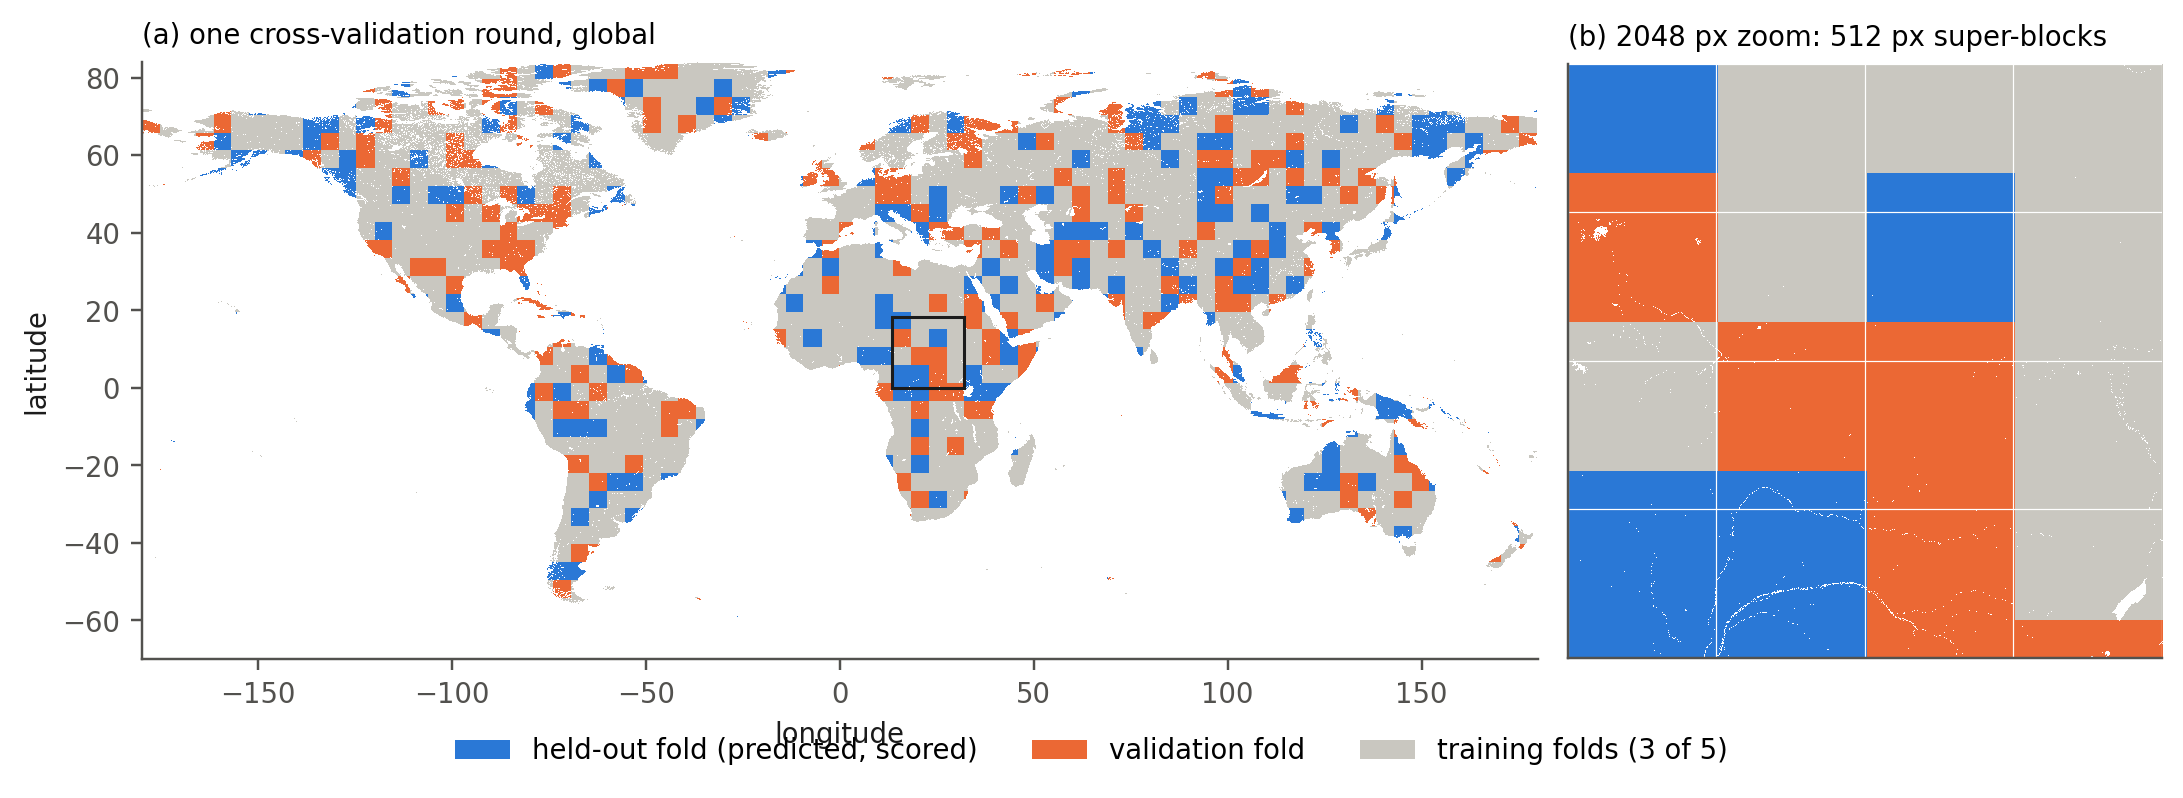
\includegraphics[width=\linewidth]{fold_roles.png}
\caption{One cross-validation round, drawn on land: fold 1 held out (blue), fold 2 validating
(orange), folds 3--5 training (grey). (b) zooms into central Africa, where the white lines are
the 512\,px super-block boundaries. The five rounds rotate the roles, so every land pixel is
held out exactly once.}
\label{fig:folds}
\end{figure}

%=====================================================================================
\section{Location encoder}
\label{sec:locenc}
%=====================================================================================

Position enters as learned features of longitude $\lambda$ and latitude $\phi$, computed per
pixel, following \citet{russwurm}: spherical-harmonic basis functions passed through a sinusoidal
representation network. The encoder lets the model represent residual geographic variation, such
as policy regimes or cultural practices, that the covariates do not measure.

\paragraph{Spherical harmonics.} With $\varphi=\lambda+180^\circ$ and $\vartheta=\phi+90^\circ$
(in radians), the encoder evaluates the real spherical harmonics $Y_\ell^m(\varphi,\vartheta)$
analytically for $\ell=0,\dots,L-1$ and $m=-\ell,\dots,\ell$ with $L=10$ Legendre degrees. That
gives a smooth, periodic, pole-consistent basis of $L^2=100$ features.

\paragraph{SIREN.} The 100 features pass through a sinusoidal network \citep{siren} with two
hidden layers of 64 units. The hidden layers compute $\sin(\omega_0(Wx+b))$, with $\omega_0=30$ in
the first layer and $1$ after it, and SIREN initialisation. A linear layer then maps to 8 output
channels. The encoder has 11,144 parameters. It is trained jointly with the rest of the network by
the same optimiser; the learning rate in its own configuration block is not used. Its 8 channels
are appended to the static inputs and repeated over the three time steps.

%=====================================================================================
\section{Trunk model}
\label{sec:trunk}
%=====================================================================================

\paragraph{Input assembly.} At each step $s\in\{1,2,3\}$ (dates $t-10$, $t-5$, $t$) the trunk
input is the concatenation
\[
X_s = \big[\,\underbrace{\tilde\HM_s,\ \tilde c_{s,1..10}}_{11\ \text{dynamic}},\
\underbrace{\tilde e_{1..7}}_{7\ \text{static}},\ \underbrace{k_{1..12}}_{12\ \text{context}},\
\underbrace{\ell_{1..8}}_{8\ \text{position}}\,\big] \in \mathbb{R}^{38\times128\times128},
\]
in which the static, context and position blocks are identical at the three steps.

\paragraph{ConvLSTM.} Four stacked ConvLSTM layers \citep{convlstm}, each with 64 hidden
channels, $3\times3$ kernels, padding 1, dilation 1 and bias. For layer $l$ at step $s$, with
input $X^{(l)}_s$ (the data for $l=1$, the previous layer's hidden state otherwise),
\begin{align*}
[\,i,f,o,g\,] &= W^{(l)} * [X^{(l)}_s,\ h^{(l)}_{s-1}] + b^{(l)}, \\
c^{(l)}_s &= \sigma(f)\odot c^{(l)}_{s-1} + \sigma(i)\odot\tanh(g), \qquad
h^{(l)}_s = \sigma(o)\odot\tanh\!\big(c^{(l)}_s\big),
\end{align*}
where $*$ is a $3\times3$ convolution producing $4\times64$ channels and the states start at
zero. The trunk output is the last layer's hidden state at the last step,
$H=h^{(4)}_3\in\mathbb{R}^{64\times128\times128}$. The trunk has 1,120,768 parameters.

\paragraph{Receptive field.} Each layer and each step widens the field by one pixel, so $H$ at a
pixel depends on a $13\times13$ window, a radius of 6\,px. This was checked by back-propagating
from a single output pixel. The heads add one more pixel. Everything the model knows about
the landscape beyond $\pm7$\,px comes from the context channels and the location encoder, which
is why those are precomputed on the full raster.

%=====================================================================================
\section{Quantile heads}
\label{sec:heads}
%=====================================================================================

For each horizon $h$ a separate decoder branch reads $H$, following the multi-horizon design of
\citet{wen}. A branch has two heads, each a $3\times3$ convolution with ReLU followed by a
$1\times1$ convolution. Together they emit a monotone spline quantile function in the sense of
\citet{gasthaus}, built from non-negative increments as in \citet{park}. Here the spline is
linear between knots, which is what gives the CRPS a closed form (Section~\ref{sec:loss}).

\paragraph{Location head.} $g_h:\ 64\to64\to1$ channels (36,993 parameters per horizon). Its
output is added to the base-year HM, giving the median
\[
m_h = x_0 + g_h(H).
\]
The output convolution is initialised to zero, so the untrained model forecasts exact
persistence and ``nothing changes'', the right answer for most of the map, costs nothing to
express.

\paragraph{Shape head.} $s_h:\ 64\to32\to14$ channels (18,926 parameters per horizon), emitting
raw values $r_{h,1},\dots,r_{h,14}$. The output weights are initialised to zero and the bias to
$\log p_k$, where $p_k$ are the standard-normal bin probabilities of the knot grid. Under the
parameterisation below the initial increments are therefore $(|\log p_k|+10^{-4})\,c$, which are
nearly equal at 0.0028--0.0039\,HM per bin: an untrained ladder with a 95\% width of about
0.028\,HM and a full span of about 0.047\,HM.

\paragraph{Knot grid.} The quantile function is represented on 15 fixed quantile levels
\[
\mathbf{u} = (0,\ 0.001,\ 0.005,\ 0.025,\ 0.05,\ 0.10,\ 0.25,\ 0.50,\ 0.75,\ 0.90,\ 0.95,\
0.975,\ 0.99,\ 0.999,\ 1),
\]
denser in the tails, and containing 0.025, 0.5 and 0.975 exactly, so the published interval and
median are read directly off knots.

\paragraph{The ladder.} In standardised units, the increments are
\[
\delta_k = \big(|r_{h,k}| + 10^{-4}\big)\, c, \qquad c = \frac{w_0}{n_{95}} = \frac{0.065}{8},
\]
with $n_{95}=8$ the number of bins spanning $[0.025,0.975]$. The constant $c$ is a \emph{unit}
(0.00125\,HM per unit of $|r|$), not a normalisation: without it the absolute scale of the raw
outputs, which earlier head families passed through a softmax, would be the width, and the
untrained ladder would start about 330 times too wide. With cumulative sums
$v_0=0$, $v_k=\sum_{j\le k}\delta_j$, the knot values are
\[
Q_h(u_k) = \operatorname{clip}\!\Big(m_h + v_k - v_7,\ \tfrac{0-\mu_{\HM}}{\sigma_{\HM}},\
\tfrac{1-\mu_{\HM}}{\sigma_{\HM}}\Big),
\]
so the median ($u_7=0.5$) is $m_h$ and the knots are clipped to the physical range
$\HM\in[0,1]$. $Q_h$ is the linear interpolant of these knot values. If the 95\% span
$Q_h(0.975)-Q_h(0.025)$ would fall below $3\times10^{-5}$\,HM, all increments are scaled up to
reach it, so a zero-width forecast cannot be emitted.

\paragraph{Properties.}
\begin{itemize}
\item \emph{Monotone by construction.} Every $\delta_k>0$, so $Q_h$ is non-decreasing and
  quantiles cannot cross.
\item \emph{Free width.} There is no separate scale channel and no coupling across horizons; each
  horizon's width emerges from its own increments.
\item \emph{Bounded support.} Without tail parameters the distribution is supported on
  $[Q_h(0),Q_h(1)]$. The far tails are carried by the two outermost bins, of probability 0.001
  each, rather than by an unbounded extension. This is the structural difference from E1v, which
  appends two learned exponential tail rates on $-\log(1-\HM)$ support.
\item \emph{Exact derived quantities.} The mean is exact because $Q_h$ is linear on each segment:
  $\E[Y]=\int_0^1 Q_h(u)\,du = \sum_k \tfrac12\big(Q_h(u_k)+Q_h(u_{k+1})\big)(u_{k+1}-u_k)$. The
  CDF and the PIT come from inverting the interpolant, and the implied density is
  piecewise constant, $(u_{k+1}-u_k)/(Q_h(u_{k+1})-Q_h(u_k))$ (Figure~\ref{fig:density}).
\end{itemize}

\paragraph{Outputs.} Per pixel and horizon the network therefore emits 15 numbers. From them it
derives the triple published beside the quantile function: \emph{lower} $=Q_h(0.025)$,
\emph{central} $=\E[Y]$ (the mean, not the median) and \emph{upper} $=Q_h(0.975)$. Because the
residual is right-skewed, the published central need not lie at the midpoint of the interval.

\emph{Implementation note.} The network module also instantiates the lower/upper heads of the
superseded three-output model (147,976 parameters). They are never called on this path, receive
no gradient and keep their initial values; they sit in the checkpoint but play no role in any
output.

\begin{figure}[t]
\centering
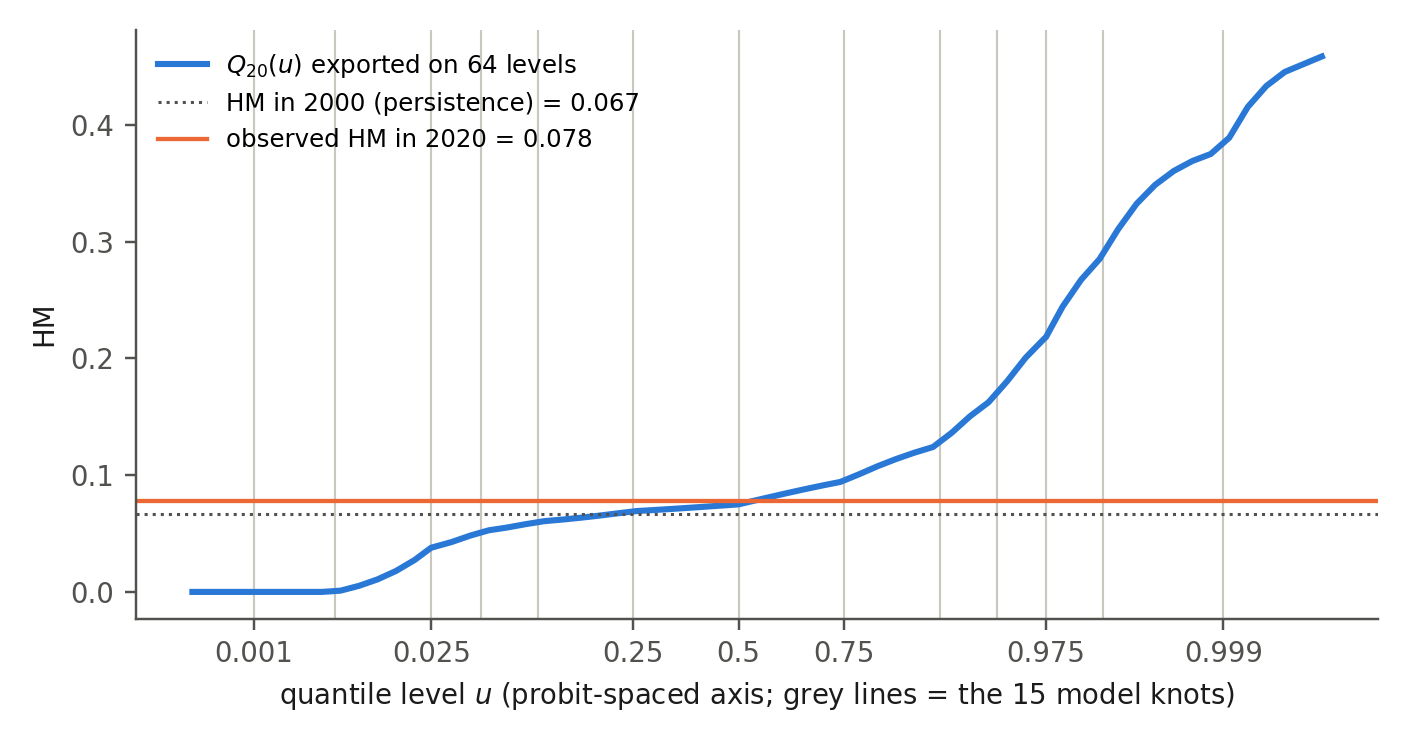
\includegraphics[width=0.82\linewidth]{quantile_ladder.png}
\caption{One pixel's predicted quantile function at +20 years (hindcast, target 2020), as
exported on 64 levels. Grey lines mark the model's 15 knots. The function is linear in $u$
between knots, which appears curved on this probit-spaced axis. Below $u\approx0.004$ the ladder
is clipped at $\HM=0$. For this pixel $Q(0.025)=0.038$, median $0.075$ and $Q(0.975)=0.218$,
against 0.067 at the base year and 0.078 observed.}
\label{fig:ladder}
\end{figure}

\begin{figure}[t]
\centering
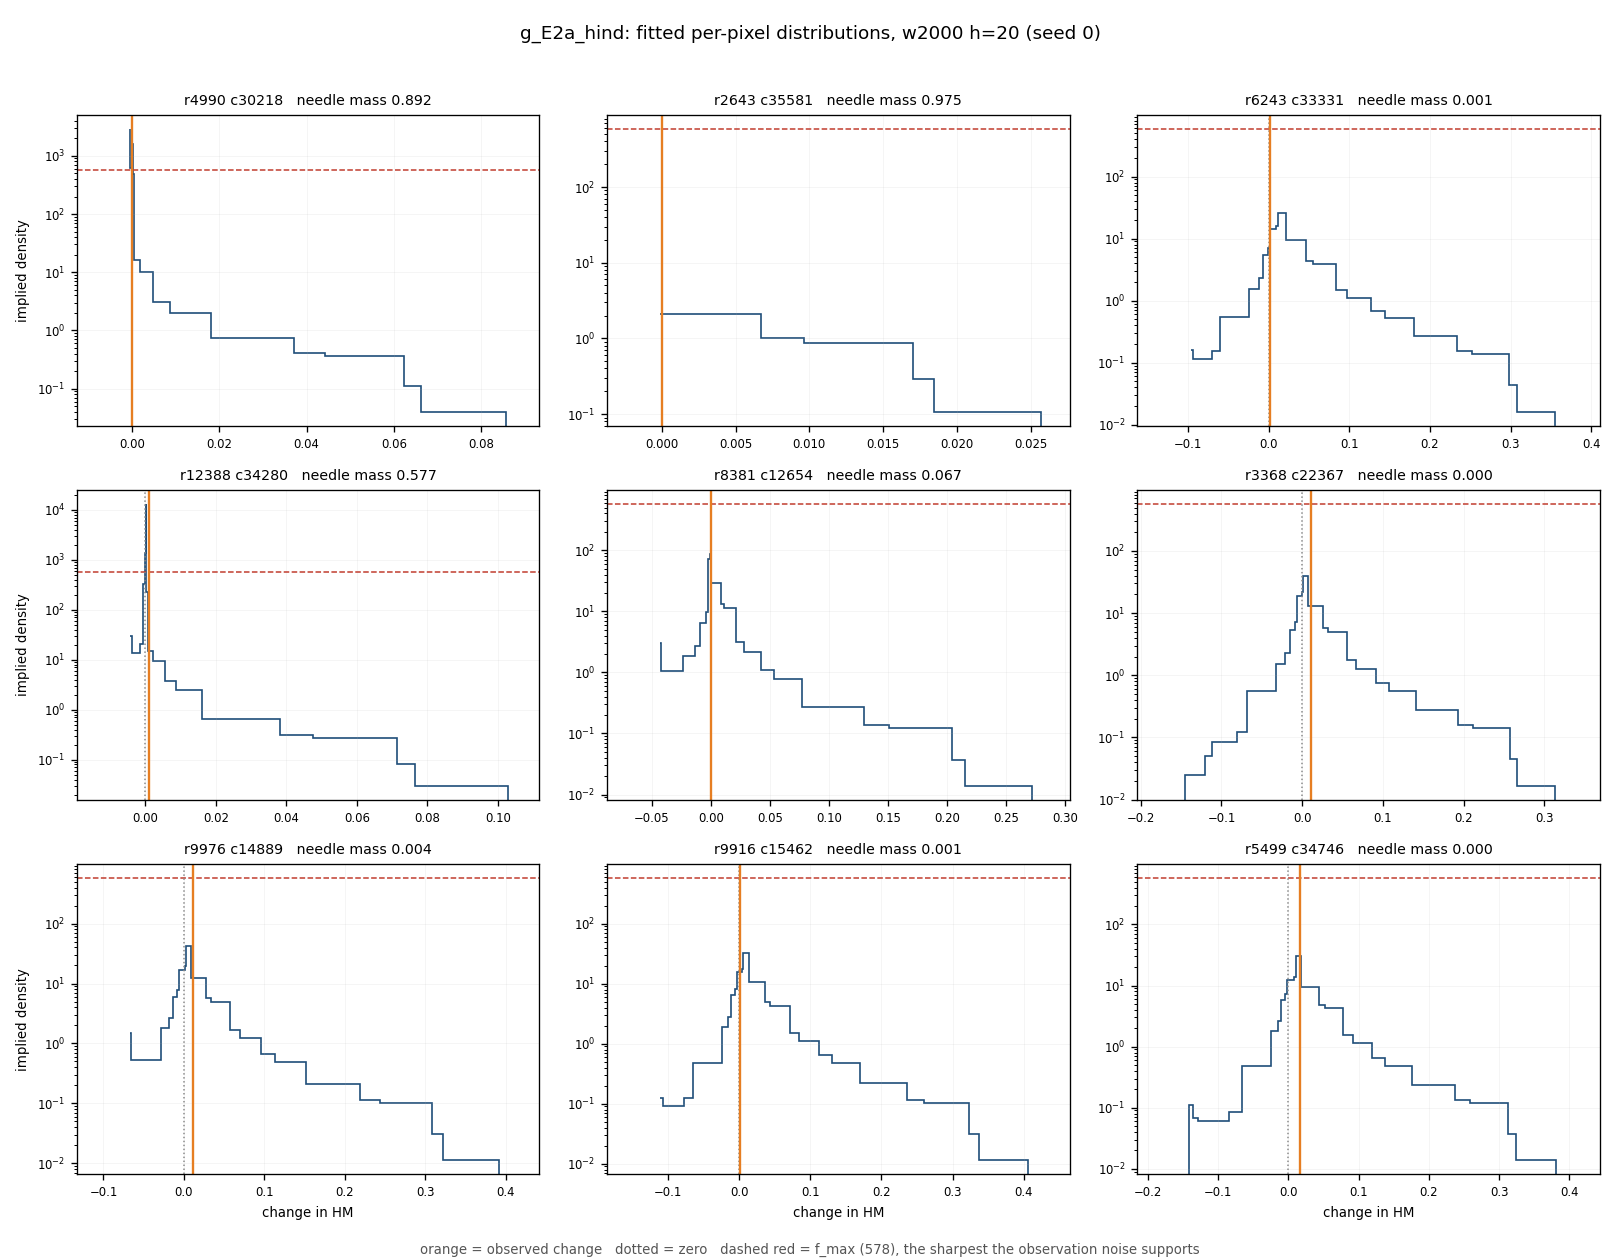
\includegraphics[width=\linewidth]{densities_g_E2a_hind.png}
\caption{Implied predictive densities of HM \emph{change} at +20 years for nine pixels on a
log axis, with the observed change marked in orange. The densities are piecewise constant because
$Q$ is piecewise linear. ``Needle mass'' and the dashed $f_{\max}=578$ reference are diagnostics
for over-sharp segments, discussed in Section~\ref{sec:eval}.}
\label{fig:density}
\end{figure}

%=====================================================================================
\section{Loss function}
\label{sec:loss}
%=====================================================================================

\paragraph{Objective.} The model minimises the CRPS \citep{gneiting}, written as the integral of the pinball
loss over quantile levels:
\[
\mathrm{CRPS}(Q,y) = 2\int_0^1 \rho_u\big(y-Q(u)\big)\,du, \qquad
\rho_u(e) = e\,\big(u-\mathbb{1}[e<0]\big).
\]
The CRPS is a strictly proper scoring rule, so it trains location, width and shape together.
Unlike the log score it has bounded influence per pixel. An earlier phase measured a Gaussian
log-likelihood inflating fitted widths by up to $7\times$ on this data, whose residual kurtosis
runs from about $10^3$ to $2\times10^4$.

\paragraph{Closed form.} On a segment $[u_k,u_{k+1}]$ where $Q$ is linear, the error
$e(u)=y-Q(u)$ is linear and non-increasing in $u$. It changes sign at most once, at
$u^*=u_k+t^*(u_{k+1}-u_k)$ with $t^*=\operatorname{clip}\big((y-Q_k)/(Q_{k+1}-Q_k),0,1\big)$.
On each side of $u^*$ the integrand $\rho_u(e(u))$ is a quadratic in $u$, so the segment
integral is exact. The implementation writes it as a three-point Simpson evaluation, which is
exact for quadratics, and sums the segments:
\[
\mathrm{CRPS}(Q,y) = 2\sum_{k=0}^{13}\Big[\,I_k(0,t^*_k;\,0) + I_k(t^*_k,1;\,1)\,\Big],
\]
where $I_k(a,b;\iota)$ integrates $e(u)\,(u-\iota)$ over the part of segment $k$ between $a$
and $b$. No quadrature nodes or approximation are involved. The implementation is checked
against a dense numerical reference that shares no code with it.

\paragraph{Reduction.} The CRPS is computed in standardised units, and one standardised unit
equals $\sigma_{\HM}$ HM. For each horizon it is averaged over valid pixels in the batch
(Section~\ref{sec:transform}); a horizon with no valid target in the batch contributes 0. The
four horizon means are then averaged with equal weight:
\[
\mathcal{L} = \tfrac14\sum_{h}\ \frac{\sum_{i}\,\mathbb{1}_i\,\mathrm{CRPS}(Q_{h,i},y_{h,i})}{\max\big(1,\sum_i \mathbb{1}_i\big)}.
\]
That is the whole objective. The code's other terms (MSE on the mean, SSIM, a Laplacian pyramid
and a histogram loss) all have weight 0 in production. There is no sample reweighting, because
tiles are drawn uniformly, and no weighting across quantile levels.

%=====================================================================================
\section{Model training}
\label{sec:training}
%=====================================================================================

\paragraph{Sampling.} An epoch draws 100 tiles from the training pool, in batches of 8 (13
steps per epoch). For each tile:
\begin{itemize}
\item the position is uniform over the admissible lattice positions (hindcast) or over the whole
  grid (forecast model);
\item the base year is drawn uniformly from $\{2000, 2005, 2010, 2015\}$, independently per tile;
\item a tile with no finite target is redrawn, up to ten times.
\end{itemize}
Because 65.6\% of lattice tiles contain no land, redraws are common. About 1.5\% of samples
($0.656^{10}$) still come back empty and contribute nothing to the loss.

\paragraph{Optimisation.} The model is implemented in PyTorch \citep{pytorch} with PyTorch
Lightning. Adam with learning rate $10^{-3}$, $\beta=(0.9,0.999)$ and no weight
decay; constant learning rate; no gradient clipping; float32 precision. The backward pass is
manual and end to end: the CRPS gradient reaches the heads, the trunk and the location encoder.
The run aborts if any weight becomes non-finite at the end of an epoch. Training lasts 150 epochs,
1,950 optimiser steps.

\paragraph{Validation and the weights used.} Each epoch the model is scored on the validation
fold's grid tiles (base year 2000, all four horizons), and the validation CRPS
(\code{val\_crps}) is logged and monitored. The weights that predict are \emph{not} the
best-validation checkpoint: they are the element-wise mean of the weights at the end of each of
the last 20 epochs (131--150), which damps optimisation noise. Held-out folds play no part in any
training decision.

\paragraph{Reproducibility and cost.} All random number generators are seeded with 42
(Python, NumPy, PyTorch, data-loader workers). On one RTX A5000 (24\,GB), training takes about
23 minutes per model. A full hindcast fold, training plus global prediction, took 103.5--106.8
minutes with two folds running concurrently on two GPUs.

\begin{table}[h]
\centering\small
\setlength{\tabcolsep}{4pt}\begin{tabular}{@{}lp{4.1cm}@{\hspace{1em}}lp{4.3cm}@{}}
\toprule
Setting & Value & Setting & Value \\
\midrule
tile size & 128\,px & optimiser & Adam, lr $10^{-3}$, no decay \\
batch size & 8 & schedule / clipping & none / none \\
tiles per epoch & 100 (13 steps) & epochs & 150 (1,950 steps) \\
base years (training) & 2000--2015, uniform & weights used & mean of last 20 epochs \\
validation & fold $v$, stride 1024, base 2000 & monitor & \code{val\_crps} \\
trunk & ConvLSTM $4\times64$, $3{\times}3$ & heads & location $64{\to}64{\to}1$, shape $64{\to}32{\to}14$ \\
location encoder & SH $L=10$, SIREN 2$\times$64, 8 out & knots & 15 (14 bins) \\
parameters (used) & 1,355,588 & seed & 42 \\
\bottomrule
\end{tabular}
\caption{Training configuration of E2a. These are the argparse defaults of
\code{scripts/train\_lightning.py}, so a run with no model flags trains E2a.}
\label{tab:hparams}
\end{table}

%=====================================================================================
\section{Global prediction}
\label{sec:global}
%=====================================================================================

\paragraph{Tiling and blending.} The grid is covered by $128\times128$ tiles at a stride of
64\,px, so every interior pixel is predicted by four tiles. Within a tile, each pixel's weight is
its Euclidean distance to the tile edge (a distance transform, zero on the border and on invalid
pixels). Each output quantity is accumulated as $\sum w\,\hat q$ and divided by $\sum w$. Every
quantile level is blended with the same weights. A weighted average of non-decreasing sequences
is non-decreasing, so the blended result is still a valid quantile function, and because 0.025
and 0.975 lie on the export grid, the blended lower and upper rasters equal the blended quantile
levels exactly. Pixels with invalid inputs are set to NaN in every tile. To bound memory, the
accumulators are processed in bands of 512 rows. Each band also accumulates every tile that
overlaps it, so the result is identical to an unbanded run.

\paragraph{Export grid.} The quantile function is written as a 64-band float32 GeoTIFF on a fixed
level grid, spaced approximately uniformly in normal score from $u=2.5\times10^{-4}$ to $0.9999$,
with 0.025, 0.5 and 0.975 pinned as exact levels. Each level is read off the model's 15-knot
function by linear interpolation; the level grid and the head's family and parameter count are
stored as raster tags. The three triple rasters (lower, mean, upper) are written alongside.

\paragraph{Hindcast mosaic.} Each fold model predicts every tile that overlaps its held-out fold.
The five fold rasters are then stitched in \emph{holdout} mode: each pixel is taken from the fold
that held it out. A mean of the five folds would be in sample and is never scored. The stitched
rasters cover 184,573,321 land pixels.

\paragraph{Forecast.} The forward model predicts the whole grid from base 2020. Its 16 rasters
each hold 184,608,551 valid pixels.

\paragraph{Products.} Both products are derived from these rasters without any further modelling.
\begin{itemize}
\item \textbf{COGs}, per year: \code{lower}${}=Q(0.025)$, \code{mean}${}=\E[Y]$,
  \code{upper}${}=Q(0.975)$ (these three copied bit-exactly), and \code{gt01}${}=1-F(0.1)$ and
  \code{gt04}${}=1-F(0.4)$ (from the scorer's CDF inversion). These are the probabilities of
  exceeding the natural-land ($\HM\le0.1$) and highly-modified ($\HM>0.4$) thresholds. Files are
  named \code{hm\_\{year\}\_\{variable\}.tif}. Single-band Float32, DEFLATE with
  floating-point predictor, 7 overview levels, EPSG:4326 at $0.009^\circ$.
\item \textbf{icechunk}: an array \code{hm}$(\text{year},\text{percentile},\text{lat},\text{lon})$ of
  shape $4\times64\times17111\times40000$. The values are stored as uint16 codes
  $\min(\mathrm{rint}(65535\,\mathrm{clip}(q,0,1)),\,65534)$, with scale $1/65535$ and 65535
  reserved as the fill value. Chunks are $1\times64\times256\times320$ (10\,MB, percentile axis
  whole) and shards $1\times64\times1024\times1280$.
\item \textbf{Observed store}: observed HM 1990--2020 on the same grid, encoding and chunk
  footprint, so observed and predicted tiles align.
\end{itemize}
Every delivered file is checked against its source rasters, bitwise where the encoding is exact.

\begin{table}[h]
\centering\small
\begin{tabular}{@{}lrr@{}}
\toprule
Stage (E2a production run) & Wall clock & Peak RAM \\
\midrule
hindcast: 5 folds, train + predict, 2 GPUs & 5\,h 14\,min & 36\,GiB \\
stitch (16 rasters) & 3\,h 18\,min & 36\,GiB \\
forward model: train + global predict & $\sim$3\,h 54\,min & 36\,GiB \\
score (4 window-years) & 5\,h 03\,min & 98\,GiB \\
export, per product & $\sim$2\,h 20\,min & 27--36\,GiB \\
\bottomrule
\end{tabular}
\caption{Measured costs on two RTX A5000 GPUs with 125\,GB of RAM.}
\end{table}

%=====================================================================================
\section{Model evaluation}
\label{sec:eval}
%=====================================================================================

\subsection{Protocol and metrics}

The stitched hindcast (base 2000, targets 2005--2020) is scored at every land pixel with a finite
observation. Each pixel's prediction comes from the fold model that never trained on it. The
reference forecast is \textbf{persistence}, $\hat y = x_0$. Scoring against zero would be
meaningless, since the median change is 0.0001. The metrics:
\begin{itemize}
\item \textbf{CRPS}, computed exactly for the piecewise-linear function the 64-level raster
  represents, with the flat tails beyond the outermost levels included in closed form. The CRPS
  of the point forecast $x_0$ is $|y-x_0|$, so
  \[
  \text{CRPS skill} = 1 - \frac{\overline{\mathrm{CRPS}}}{\overline{|y-x_0|}}.
  \]
\item \textbf{MSE skill} of the mean forecast, $1-\overline{(\E[Y]-y)^2}\,/\,\overline{(x_0-y)^2}$.
  The manuscript calls this forecast skill and the scorecards label it ``RMSE skill''; it is
  the MSE ratio in both.
\item \textbf{Coverage} of the central 50, 80, 95 and 99\% intervals, and their mean widths.
\item \textbf{PIT} $u^*=F(y)$, by inverting the interpolant: its mean (0.5 if centred), the
  Kolmogorov--Smirnov distance to uniform, and the tail frequencies $P(u^*<0.001)$ and
  $P(u^*>0.999)$ (0.001 each if calibrated). The far-tail excess is
  $\big(P(u^*<0.001)+P(u^*>0.999)\big)/0.002$, which is 1 when calibrated.
\item \textbf{Tail reach} $\big(Q(0.999)-Q(0.5)\big)/\big(Q(0.975)-Q(0.5)\big)$, and exceedance
  probabilities $P(\Delta>0.01)$, $P(\Delta>0.05)$ and $P(\Delta<-0.01)$ compared with observed
  frequencies.
\end{itemize}
Pooled scores average over all pixels, and 99.9\% of pixels are nearly static. So every metric is
also reported by stratum:
\begin{itemize}
\item distance to past change, in bins $[0,1]$, $(1,3]$, $(3,10]$, $(10,30]$, $(30,100]$, $(100,\infty)$\,px
  (right-closed);
\item predicted change;
\item base-year HM;
\item observed change.
\end{itemize}

\subsection{Results}

\begin{table}[h]
\centering\small
\begin{tabular}{@{}lrrrrrrrr@{}}
\toprule
Horizon & CRPS & CRPS skill & RMSE & MSE skill & cov50 & cov95 & PIT mean & PIT KS \\
\midrule
+5 yr  & 0.002980 & 0.154 & 0.01334 & 0.039 & 0.416 & 0.953 & 0.509 & 0.076 \\
+10 yr & 0.005284 & 0.266 & 0.02029 & 0.191 & 0.409 & 0.961 & 0.560 & 0.123 \\
+15 yr & 0.007225 & 0.302 & 0.02639 & 0.233 & 0.449 & 0.948 & 0.553 & 0.120 \\
+20 yr & 0.008905 & 0.302 & 0.03113 & 0.243 & 0.466 & 0.896 & 0.552 & 0.115 \\
\bottomrule
\end{tabular}
\caption{Out-of-sample hindcast scores of E2a over all 184,573,321 land pixels, base year 2000.
CRPS and RMSE are in HM units.}
\label{tab:scores}
\end{table}

The model improves on persistence at every horizon, by 15\% in CRPS at +5 years rising to 30\% at
+15 and +20 years. Skill is carried mostly by pixels near past change: CRPS skill at +20 years
falls from 0.42 within 1\,px of past change to 0.12 at 30--100\,px (Figure~\ref{fig:bands}a).

Beyond 100\,px it rises again, to 0.30, and there the point forecast also beats persistence (MSE
skill 0.031). That is a long-horizon result only: at +5 years the same band loses to persistence
(CRPS skill $-0.181$, MSE skill $-0.0185$).

\begin{figure}[t]
\centering
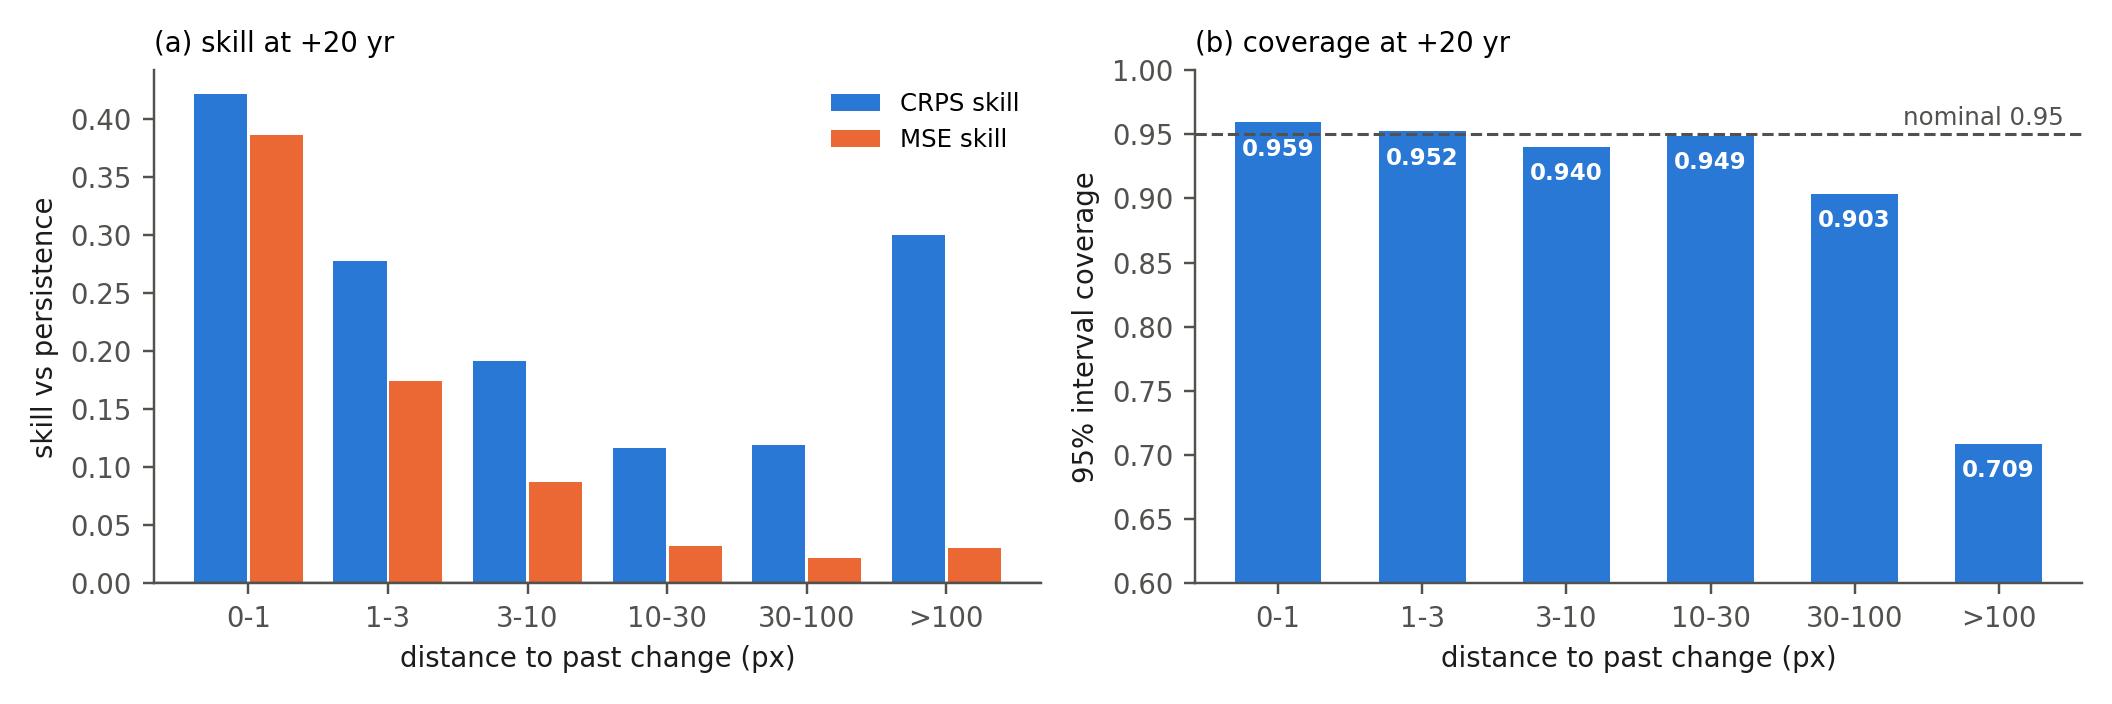
\includegraphics[width=\linewidth]{band_skill.png}
\caption{Skill and calibration by distance to past change at +20 years. (a) CRPS and MSE skill
against persistence. (b) Coverage of the 95\% interval; the far field ($>$100\,px, 33.6\,M
pixels) covers 0.709 against 0.95.}
\label{fig:bands}
\end{figure}

\paragraph{Calibration and known limitations.}
\begin{itemize}
\item \textbf{Far-field intervals are too narrow.} Beyond 100\,px from past change at +20 years,
  the 95\% interval covers 70.9\% of observations and 12.7\% of pixels exceed their predicted
  99.9th percentile, against 0.1\% nominal. Pooled over all land this appears only as a +20-year
  coverage of 0.896 and a far-tail excess of 22.3. It follows from the bounded support
  (Section~\ref{sec:heads}): the distribution cannot reach beyond its outermost knots.
\item \textbf{The distribution is centred slightly low.} The PIT mean is 0.51--0.56, and the PIT
  histogram shows recurring spikes near 0.22, 0.52, 0.77 and 0.95 at every horizon
  (Figure~\ref{fig:pit}).
\item \textbf{Central intervals are too narrow}: 50\% coverage is 0.41--0.47 and 80\% coverage
  0.74--0.77, while 95\% coverage is close to nominal except at +20 years.
\item \textbf{The lower far tail is over-populated}: $P(u^*<0.001)$ is 0.0095--0.013.
\end{itemize}
The implied densities are very sharp at many pixels (Figure~\ref{fig:density}). At global scale
this is dominated by the physical boundary $\HM=0$, on which most wilderness sits: 69--78\% of
pixels are flat on a bound, while the fraction with a degenerate segment away from the boundary
is 0.000 at three horizons and 0.029 at +20 years.

\begin{figure}[t]
\centering
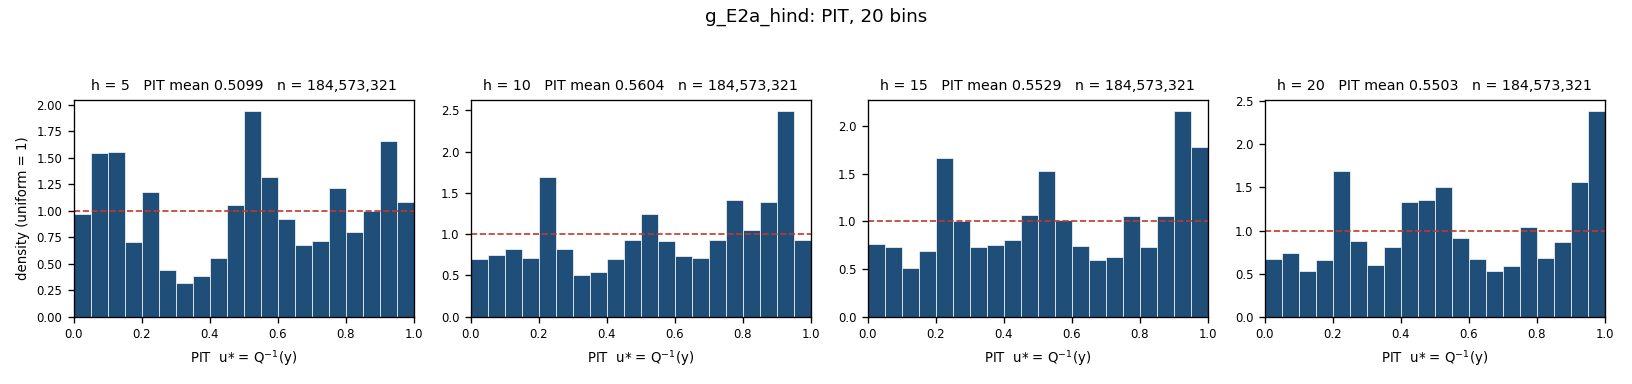
\includegraphics[width=\linewidth]{pit_g_E2a_hind.png}
\caption{PIT histograms of the hindcast, 20 bins, all land pixels. A calibrated forecast is flat
at 1.}
\label{fig:pit}
\end{figure}

\begin{figure}[t]
\centering
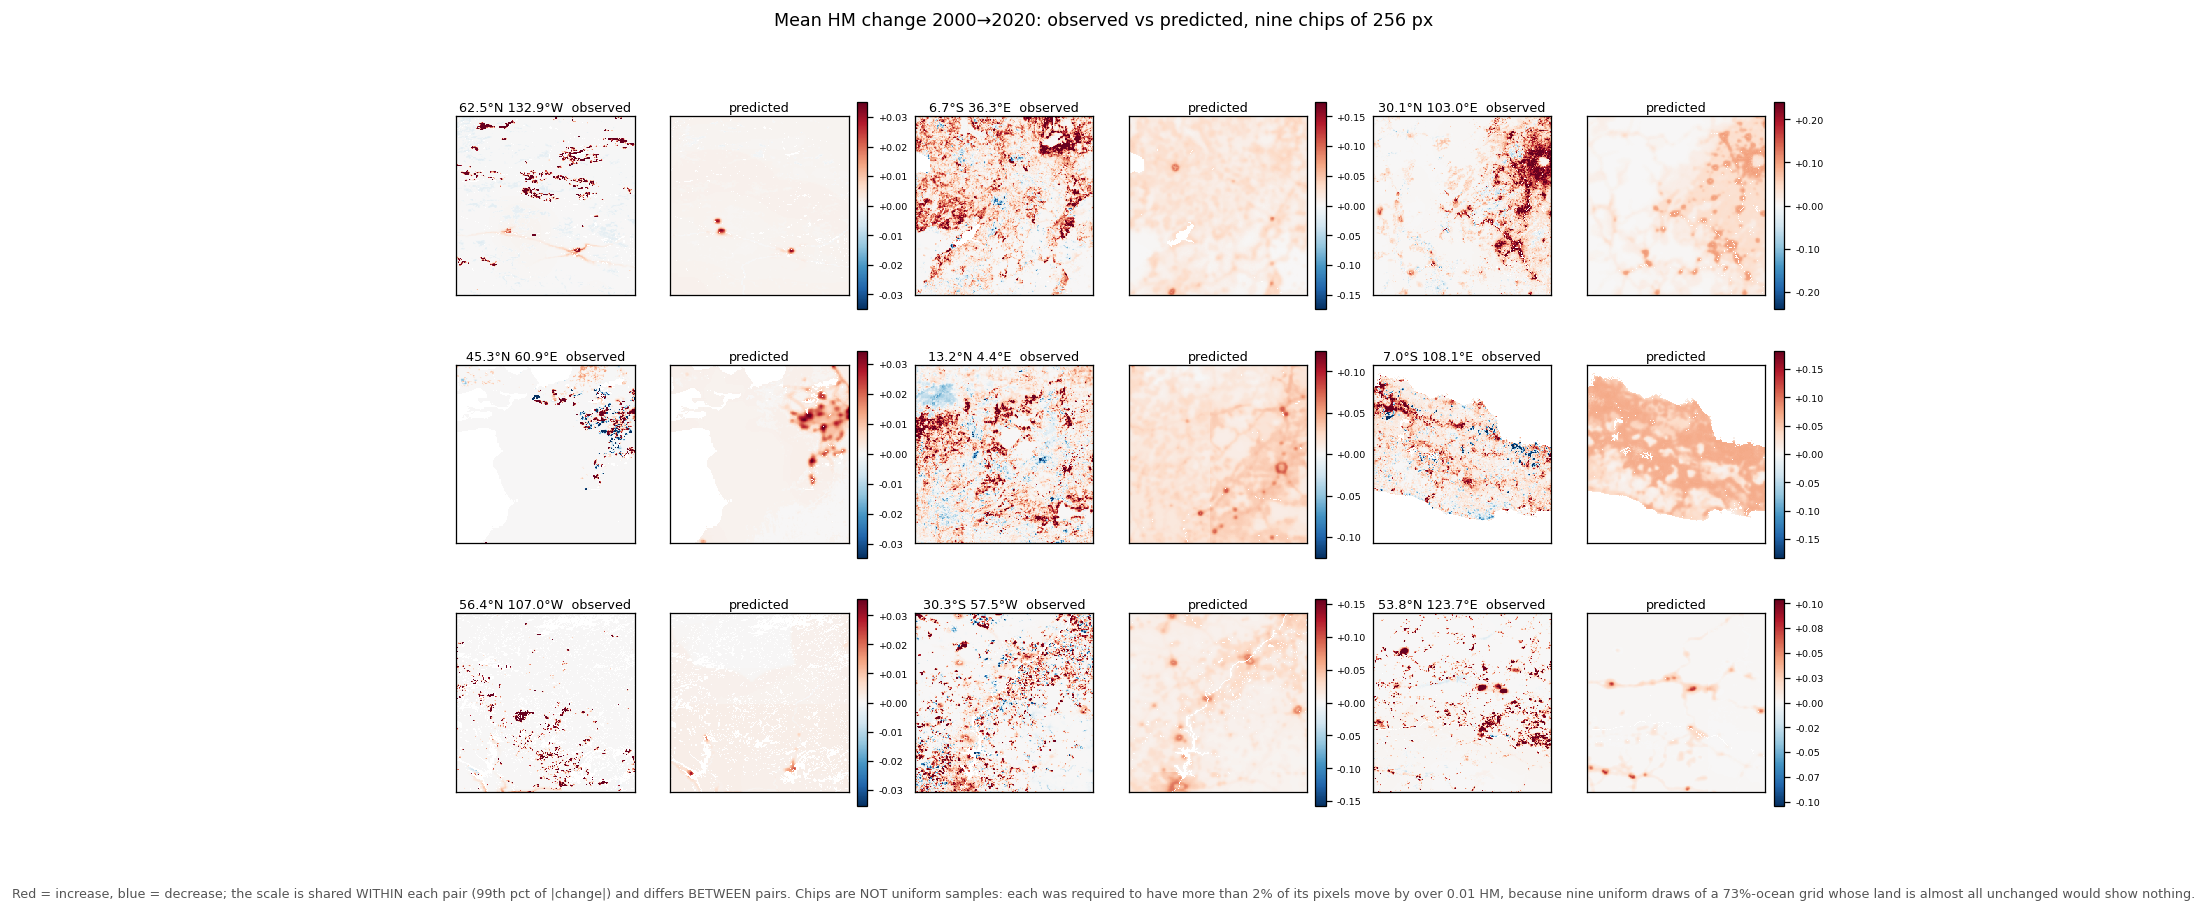
\includegraphics[width=\linewidth]{chips_g_E2a_hind.png}
\caption{Observed against predicted mean change 2000$\to$2020 for nine $256\times256$\,px tiles,
each required to have more than 2\% of its pixels change by over 0.01\,HM. The predicted field
is the mean $\E[Y]-x_0$ and is smoother than the observation, as a mean should be.}
\label{fig:chips}
\end{figure}

\subsection{The learned-tails ablation: E2a against E1v}
\label{sec:ab}

E1v is E2a plus two learned exponential tail rates on $-\log(1-\HM)$ support (17 parameters per
horizon), trained and scored with the identical global protocol.
\begin{center}\small
\setlength{\tabcolsep}{4pt}\begin{tabular}{@{}p{6.2cm}rr@{}}
\toprule
 & E1v (17 p) & E2a (15 p) \\
\midrule
CRPS skill, pooled, +5 / +10 yr & 0.157 / 0.266 & 0.154 / 0.266 \\
CRPS skill, pooled, +15 / +20 yr & 0.300 / 0.298 & 0.302 / 0.302 \\
95\% coverage, pooled, +20 yr & 0.965 & 0.896 \\
far-tail excess, pooled, +20 yr (1 = calibrated) & 7.9 & 22.3 \\
\midrule
$>$100\,px, +20 yr: CRPS skill & 0.217 & 0.300 \\
$>$100\,px, +20 yr: MSE skill & $-0.007$ & $+0.031$ \\
$>$100\,px, +20 yr: 95\% coverage & 0.995 & 0.709 \\
$>$100\,px, +20 yr: $P(u^*>0.999)$ & 0.0016 & 0.127 \\
\bottomrule
\end{tabular}
\end{center}
\begin{itemize}
\item \emph{Centrally the heads are indistinguishable}: pooled CRPS skill differs by at most
  0.004 and pooled RMSE by $5\times10^{-5}$.
\item \emph{Far from past change the tails trade calibration for sharpness.} Without them, the
  narrower distribution improves CRPS and the point forecast, and loses interval coverage.
\item \emph{Neither head is calibrated in the far field}, and they err in opposite directions:
  E1v conservatively, E2a overconfidently.
\end{itemize}
E2a was chosen for its simplicity and its far-field point forecast, with the far-field interval
width recorded as a known limitation.

%=====================================================================================
\appendix
\section{Reproduction}
%=====================================================================================

\paragraph{Commands.} With the argparse defaults of \code{train\_lightning.py} equal to E2a,
a single model is trained with
\begin{center}
\code{python scripts/train\_lightning.py --predict\_region config/region\_africa.geojson}
\end{center}
The full global run is driven by one script whose stages refuse to start without a passing smoke
test of the same code and configuration:
\begin{center}
\code{MODEL=E2a ALLOW\_GLOBAL=1 ./scripts/run\_global\_model.sh}
\code{smoke|hindcast|stitch|score|forecast|export\_hindcast|export\_forecast}
\end{center}

\paragraph{Artefacts.}
\begin{itemize}
\item Checkpoints: \code{models/production/E2a\_global/} (five fold models and the forward model).
\item Normalisation statistics: \code{data/conv\_spline/norm\_stats.json}. Like the checkpoints,
  it is not versioned in git and must travel with them.
\item Scorecards: \code{docs/global/scores/}.
\item Delivered products: \code{products/E2a/} and \code{products/observed/} on the project
  storage volume.
\end{itemize}

\paragraph{Where things are implemented.}
\begin{center}\small
\begin{tabular}{@{}p{4.8cm}p{10.4cm}@{}}
\toprule
Component & File \\
\midrule
data loading, normalisation, sampling & \code{scripts/torchgeo\_dataloader.py} \\
context rasters & \code{scripts/prepare\_change\_context.py},\newline \code{scripts/prepare\_hm\_context.py} \\
context channels & \code{src/models/change\_weights.py} \\
fold mask & \code{scripts/create\_validity\_mask.py}\newline \code{--folds\_only --fold\_block\_chips 4} \\
location encoder & \code{src/locationencoder/} \\
trunk and heads & \code{src/models/convlstm.py},\newline \code{src/models/spatiotemporal\_predictor.py} \\
quantile function, closed-form CRPS & \code{src/models/quantile\_pwl.py} \\
loss and training loop & \code{src/models/lightning\_module.py},\newline \code{scripts/train\_lightning.py} \\
fold orchestration, stitching & \code{scripts/run\_hindcast\_folds.py},\newline \code{src/stitch.py} \\
scoring & \code{scripts/score\_distributional\_model.py} \\
products and verification & \code{scripts/export\_products.py},\newline \code{scripts/verify\_products.py} \\
\bottomrule
\end{tabular}
\end{center}

\begin{thebibliography}{99}
\bibitem[Amatulli et al.(2018)]{amatulli}
G.~Amatulli, S.~Domisch, M.-N.~Tuanmu, B.~Parmentier, A.~Ranipeta, J.~Malczyk and W.~Jetz (2018).
A suite of global, cross-scale topographic variables for environmental and biodiversity modeling.
\emph{Scientific Data} 5, 180040.
\bibitem[Gasthaus et al.(2019)]{gasthaus}
J.~Gasthaus, K.~Benidis, Y.~Wang, S.~S.~Rangapuram, D.~Salinas, V.~Flunkert and T.~Januschowski
(2019). Probabilistic forecasting with spline quantile function RNNs. \emph{AISTATS}, 1901--1910.
\bibitem[Gneiting and Raftery(2007)]{gneiting}
T.~Gneiting and A.~E.~Raftery (2007). Strictly proper scoring rules, prediction, and estimation.
\emph{Journal of the American Statistical Association} 102, 359--378.
\bibitem[Karger et al.(2017)]{karger}
D.~N.~Karger, O.~Conrad, J.~B\"ohner, T.~Kawohl, H.~Kreft, R.~W.~Soria-Auza, N.~E.~Zimmermann,
H.~P.~Linder and M.~Kessler (2017). Climatologies at high resolution for the earth's land surface
areas. \emph{Scientific Data} 4, 170122.
\bibitem[Murakami et al.(2021)]{murakami}
D.~Murakami, T.~Yoshida and Y.~Yamagata (2021). Gridded GDP projections compatible with the five
SSPs. \emph{Frontiers in Built Environment} 7, 760306.
\bibitem[Oakleaf et al.(2024)]{oakleaf2024}
J.~R.~Oakleaf, C.~M.~Kennedy, N.~H.~Wolff et al.\ (2024). Mapping global land conversion pressure
to support conservation planning. \emph{Scientific Data} 11, 830.
\bibitem[Park et al.(2022)]{park}
Y.~Park, D.~Maddix, F.-X.~Aubet, K.~Kan, J.~Gasthaus and Y.~Wang (2022). Learning quantile
functions without quantile crossing for distribution-free time series forecasting.
\emph{AISTATS}, 8127--8150.
\bibitem[Paszke et al.(2019)]{pytorch}
A.~Paszke et al.\ (2019). PyTorch: an imperative style, high-performance deep learning library.
\emph{NeurIPS}.
\bibitem[Ru{\ss}wurm et al.(2023)]{russwurm}
M.~Ru{\ss}wurm, K.~Klemmer, E.~Rolf, R.~Zbinden and D.~Tuia (2023). Geographic location encoding
with spherical harmonics and sinusoidal representation networks. arXiv:2310.06743.
\bibitem[Shi et al.(2015)]{convlstm}
X.~Shi, Z.~Chen, H.~Wang, D.-Y.~Yeung, W.-K.~Wong and W.-C.~Woo (2015). Convolutional LSTM
network: a machine learning approach for precipitation nowcasting. \emph{NeurIPS}.
\bibitem[Sitzmann et al.(2020)]{siren}
V.~Sitzmann, J.~N.~P.~Martel, A.~W.~Bergman, D.~B.~Lindell and G.~Wetzstein (2020). Implicit
neural representations with periodic activation functions. \emph{NeurIPS}.
\bibitem[Theobald et al.(2025)]{theobald}
D.~M.~Theobald, J.~R.~Oakleaf, G.~Moncrieff, M.~Voigt, J.~Kiesecker and C.~M.~Kennedy (2025).
Global extent and change in human modification of terrestrial ecosystems from 1990 to 2022.
\emph{Scientific Data} 12, 606.
\bibitem[UNEP-WCMC and IUCN(2025)]{wdpa}
UNEP-WCMC and IUCN (2025). Protected Planet: the World Database on Protected Areas.
\bibitem[Wen et al.(2017)]{wen}
R.~Wen, K.~Torkkola, B.~Narayanaswamy and D.~Madeka (2017). A multi-horizon quantile recurrent
forecaster. NIPS Time Series Workshop, arXiv:1711.11053.
\bibitem[Zhuang et al.(2024)]{zhuang}
H.~Zhuang, X.~Liu, B.~Li, C.~Wu, Y.~Yan, L.~Zeng and C.~Zheng (2024). Mapping high-resolution
global gridded population distribution from 1870 to 2100. \emph{Science of the Total
Environment} 955, 176867.
\end{thebibliography}

\end{document}
